\documentclass[12pt,a4paper]{article}
\usepackage{graphicx}
\usepackage{placeins}
\usepackage{indentfirst}
\usepackage{polski}
\usepackage[utf8]{inputenc}
\title{Sprawozdanie z laboratorium PAMSI}
\author{Damian Oleksak}
\date{}
\begin{document}
\maketitle
\newpage

\section*{Wstęp i wyniki pomiarów}

Do rozwiązywania różnego rodzaju problemów służą odpowiednie\\ algorytmy. Do pracy algorytmu niezbędne są struktury danych, które przechowują informacje.
W zależności od charakterystyki rozwiązywanego problemu, stawiamy tym strukturom określone wymagania.
\newline

Tablice asocjacyjne przechowują dane parami, na które składają się wartość i klucz. Aby uzyskać dostęp do żądanej wartości, posługujemy się kluczem. Zależy nam na jak najbardziej efektywnym czasie dostępu do wybranej wartości. Czas zapisu mniej nas interesuje i jest zwykle dłuższy od czasu odczytu.
\newline

Tablica asocjacyjna została zrealizowana w trzech wersjach:\newline
-tablica przy użyciu std::vector;\newline
-drzewo poszukiwań binarnych;\newline
-tablica mieszająca.\newline

Sprawozdanie zawiera porównanie czasu dostępu do ostatniego elementu.
\newpage


\begin{table}[t]
\caption{Wyniki czasu dostępu do ostatniego elementu tablicy mieszającej}
\label{tab. mieszająca}
\centering
\begin{tabular}{|c|c|}
  \hline 
  LICZBA ELEMENTÓW & CZAS [us]\\
  \hline
  10 & 26 \\
  \hline
  100 & 21 \\
  \hline
    1000 & 28 \\
    \hline
      10000 & 30 \\
      \hline
        20000 & 36 \\
        \hline
          30000 & 37 \\
          \hline
            40000 & 35 \\
            \hline
              50000 & 36 \\
              \hline
                60000 & 37 \\
  \hline
\end{tabular} 
\end{table}



Wykres 1. Tablica mieszająca\\

\includegraphics[scale=0.6]{./miesz}

\newpage

\begin{table}[t]
\caption{Wyniki czasu dostępu dla drzewa poszukiwań binarnych}
\label{BST}
\centering
\begin{tabular}{|c|c|}
  \hline 
  LICZBA ELEMENTÓW & CZAS [us]\\
  \hline
  10 & 1 \\
  \hline
  100 & 2 \\
  \hline
    1000 & 15 \\
    \hline
      10000 & 41 \\
      \hline
        20000 & 88 \\
        \hline
          30000 & 150 \\
          \hline
            40000 & 217 \\
            \hline
              50000 & 276 \\
              \hline
                60000 & 319 \\
  \hline
\end{tabular} 
\end{table}



Wykres 2. Drzewo poszukiwań binarnych\\

\includegraphics[scale=0.6]{./bst}

\newpage

\begin{table}[t]
\caption{Wyniki czasu dostępu dla tablicy na std::vector}
\label{asoc}
\centering
\begin{tabular}{|c|c|}
  \hline 
  LICZBA ELEMENTÓW & CZAS [us]\\
  \hline
  10 & 16 \\
  \hline
  100 & 18 \\
  \hline
    1000 & 136 \\
    \hline
      10000 & 841 \\
      \hline
        20000 & 594 \\
        \hline
          30000 & 829 \\
          \hline
            40000 & 1209 \\
            \hline
              50000 & 1400 \\
              \hline
                60000 & 1966 \\
  \hline
\end{tabular} 
\end{table}



Wykres 3. Tablica przy użyciu std::vector\\

\includegraphics[scale=0.6]{./vec}

\newpage

Wykres 4. Zbiorcze porównanie\\

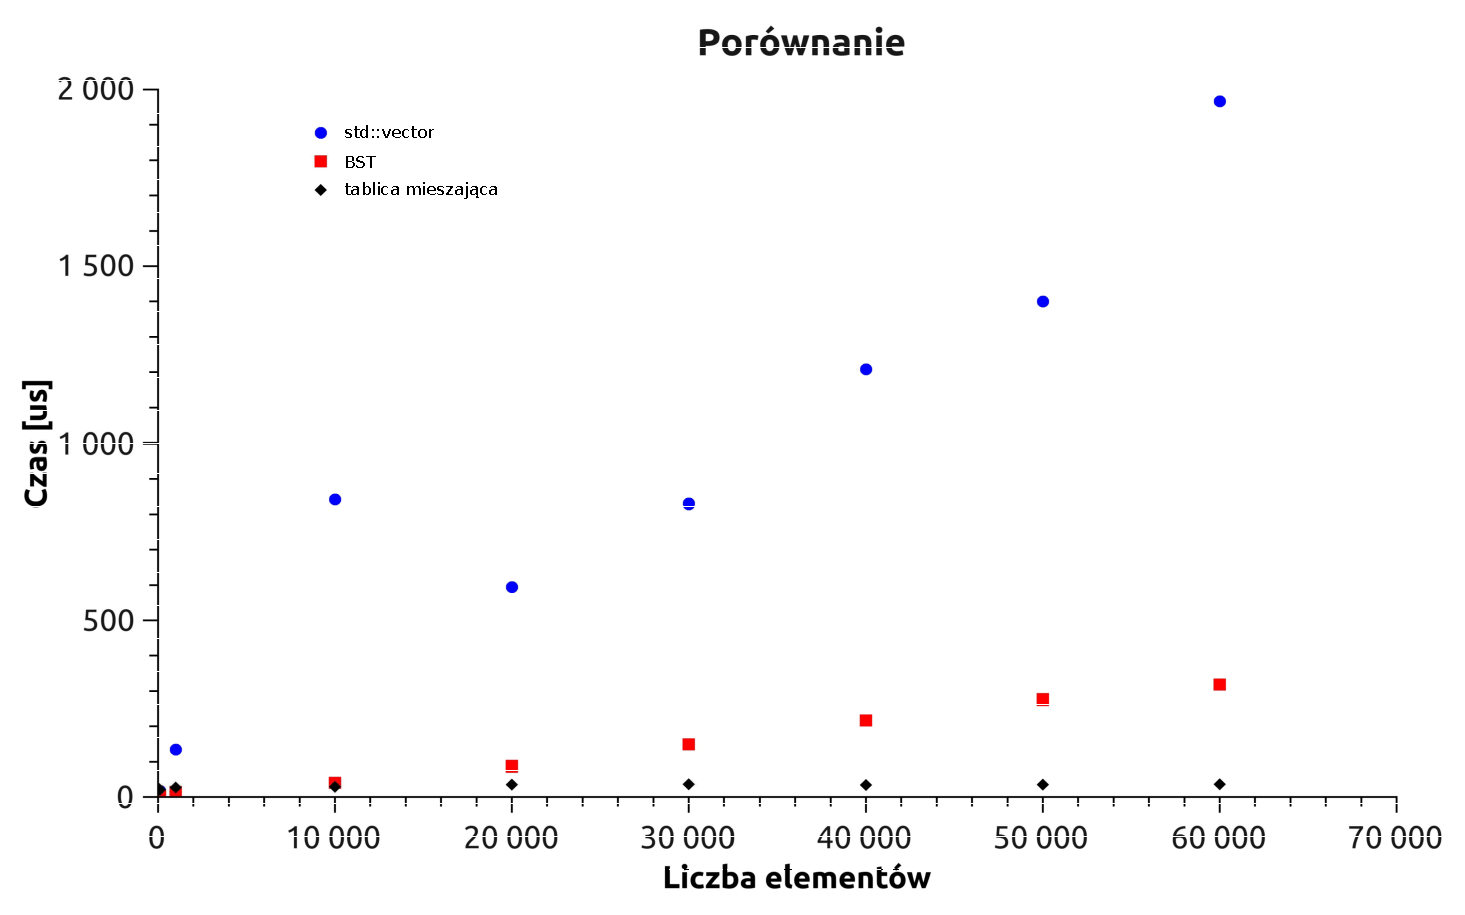
\includegraphics[scale=0.6]{./zb}

\newpage

\section*{Uwagi i wnioski}

Drzewo poszukiwań binarnych (BST) to drzewo, w którym dla każdego węzła "x" musi być spełniony następujący warunek:

Wartość każdego elementu leżącego w lewym poddrzewie węzła x jest nie większa niż wartość węzła x, natomiast wartość każdego elementu leżącego w prawym poddrzewie węzła x jest nie mniejsza niż wartość tego węzła.
\\

Przeszukiwanie odbywa się tylko wzdłuż drzewa, więc czas operacji jest proporcjonalny do jego wysokości. Przypadek optymistyczny wynosi O(logn). Gdy drzewo jest skrajnie niezrównoważone i jego wysokość jest równa liczbie węzłów, koszt operacji wynosi O(n).\\ 

Dla tablicy haszującej kluczowym elementem jest jej funkcja haszująca. Zwraca ona dla określonej wartości elementu wartość z zakresu [0,m-1], gdzie m jest rozmiarem tablicy. Funkcja ta musi być deterministyczna, tzn. zawsze dla elementu o wartości k musi zwrócić tą samą wartość.
\\

Ważne jest równomierne haszowanie, by wszystkie listy tablicy haszującej miały podobną długość. Skraca to czas wykonywania operacji słownikowych. (Najkrótszy byłby, gdyby wszystkie listy miały identyczną długość).
\\

Zaimplementowana funkcja mieszająca mnoży wartość znaku(za pomocą przesunięcia bitowego) i sumuje ją z poprzednim wynikiem. Przydzielony hasz jest wynikiem dzielenia modulo tej sumy przez rozmiar tablicy.
\\

Wyniki pomiarów obrazują, że najwydajniejszym rozwiązaniem jest tablica mieszająca. Taki wynik został osiągnięty dzięki odpowiednio dużemu rozmiarowi tej tablicy, przez co elementy rozkładają się równomiernie. Gdyby występowały kolizje, konieczne byłoby przeszukiwanie w listach. Sprawdzanie każdego elementu wydłuża czas liniowo, więc dla bardzo licznych zbiorów czas dostępu znacząco by się wydłużył. Za przykład może posłużyć tablica o rozmiarze 7. Czas odczytu wyniósł 769 us dla 30000 elementów. W porównaniu do 37 us, gdy rozmiar tablicy przekraczał liczbę elementów, różnica jest zauważalna. \\

Zwykła tablica asocjacyjna bez funkcji mieszającej ma najdłuższe czasy odczytu, gdyż przeszukiwanie odbywa się po każdym elemencie.
\end{document} 
